In this section, we present models used in our work. For ease of reference, notations used in this paper are listed in table~\ref{tablen}.

\begin{table}[!h]
\caption{Formulae Notations }
\label{tablen}
\centering
\begin{tabular}{|c|c|}

\hline
\textit{\textbf{Parameter}}&\textit{\textbf{Description}}\\
\hline
\hline
$U$&Customer satisfaction\\
\hline
$\alpha$ \& $\beta$&Coefficients in utility function\\
\hline
$p$&Service price/Revenue\\
\hline
$i$&The index of customers and VMs\\
\hline
$U$& Total service time for a user\\
\hline
$V$&Customer value\\
\hline
$D$&Degree of churn\\
\hline
$P$&A particular customer consumption history\\
\hline
$S$&Sample space of all customer\\
\hline
$r$&Churn rate\\
\hline
$RC$&Retention cost\\
\hline
$RI$&Retention cost index\\
\hline
$\varphi$&Retention cost coefficient\\
\hline
$j$&The index of PMs\\
\hline
$O$&Capacity of VM\\
\hline
$Q$&Capacity of PM\\
\hline
$C$&Cost of running PM\\
\hline
$n$&Number of customers or VMs\\
\hline
$b$ \& c& Overhead coefficient\\
\hline
$H$&Overhead\\
\hline
$\theta_{ij}$&$VM_i$ is placed on $PM_j$\\
\hline
\end{tabular}
\end{table}

\subsection{Churn Aware Cloud Computing Framework}

%In our paper, we are not only talk about cloud services and how to assign those virtual machines to physical machine and get the maximal profit but also consider about the customers churn rate and make a retention action to reduce churn rate so that cloud provider can get a maximal profit from serving clients and meanwhile customers could feel better from that. Figure \ref{frame} reveals this basic frame.

Churn aware cloud computing framework is presented in Figure \ref{frame}. We consider a cloud computing framework where cloud users submit their requests with SLA constraints on capacity and cost of virtual machines. Both capacity and cost are associated with the profit of cloud service providers. Furthermore, cloud users desire higher capacity and their profit improves with increase in capacity for the same or lower price.  The historical user data along with current SLAs are used to allocate resources for users and allocated resources in the form of VMs are available for use by remotely accessing the physical machines. A set of designated physical machines known as master nodes can instantiate virtual machines satisfying the resource allocation and then place them on worker nodes (physical machines). Process of allocation and placement of resources for cloud users is shown in Figure~\ref{flowchart}. For existing users, resource allocation and placement is done by consulting the historical user data. First, churners among users are identified and then degree of churn is computed for each churners. Furthermore, based on degree of churn, retention index is computed that decides on appropriate retention action for customers. Resource allocation is determined based on both retention action and contract SLA. Finally, VM placement algorithm assigns VMs to physical machines.

%and process the jobs at the same time. From this theory, a Master-Node for managing those virtual machines and jobs is essential. Unlike physical infrastructure distribution, our model just talks about in one physical machine. In our model, each Worker-Node could be a virtual machine as well as Master-Node, both Master and Worker-Node utilize the hardware from physical resources.  and finally, VMs with allocated resources are assigned to a set of physical machines that users can access and use


%The procedure is customer s log into cloud provider system, if a customer is not the first time to use this service, this customers database should have the records of this customer, after logged in customers can sent the jobs to the cloud and declare how much they are going to pay for the jobs they submitted, customers database has already stored customers records such as  customers' value and degree of churn, so the cloud provider will tell the customers the response time and amendatory response time based on retention action and customers' information, once cloud provider knew the amendatory response time, system will create virtual machines for these jobs and assign these virtual machines to different physical machines. Finally, system will return the results to the customers. In this frame, we will use twice utility function which can help us calculate the response time. In next section, we will detailed introduce what happens on Service-Level Agreements (SLA). 


%\subsection{Master-Worker Model}
%Master-Worker Node model is adopted in our work. In a physical machine of cloud computing, a cloud service provider has a certain amount of hardware infrastructure, but clients just can use part of them which meaning one virtual machine will be given to each customer based on her requirements and money she needs to pay. Once cloud provider knew a particular customer requirement, system will assign some resource from physical machine to the applications which is a virtual machine created. 

\begin{figure}[!h]
\centering
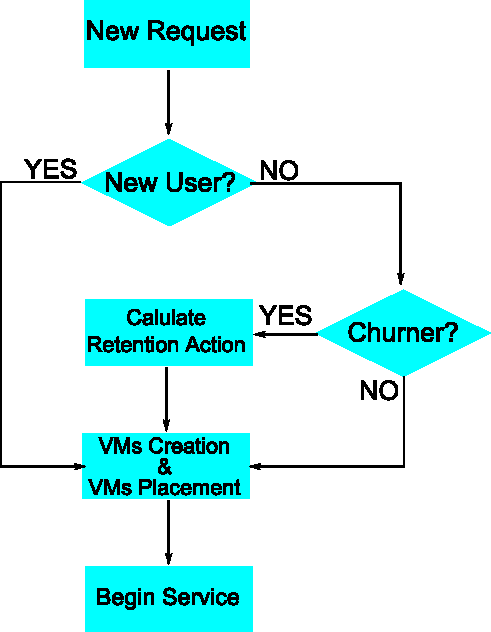
\includegraphics[scale=0.75]{pic/flowchart.pdf}
\caption{Flowchart showing process of allocation and placement of resources}
\label{flowchart}
\end{figure}




\subsection{Revenue and Cost}
 Cloud service provider charges a price $p$ for capacity $O$ according to following utility function  
\begin{equation}
 p= \alpha O+\beta
\label{eq:reveneue}
\end{equation}
where $\alpha$ and $\beta$ are coefficients of utility function.


Furthermore, there is a fixed cost $C_j$ associated with some physical machine $j$ if it is turned on.

%Retention Action can save more customers who want to switch to other companies. However, the profit of business is still in firth place of considering. So we will analysis retention action and profit in this section.
\subsection{Retention Action}
In this section, first, we present the theory of user satisfaction using a economics model that explains the motivation behind retention action (RA). The central idea behind RA is to improve satisfaction levels of churners by offering them more capacity for the same price. 
%The first mentioned of two is a fixed value retention action in cost while the second one is various values that should be based on some economics principles. So in the next section we will talk about these two schemes respectively.

%For a company or a cloud service provider, they need to do something to try to change a churner to non-churner. They can give something discount or provide extra benefits to their customers.
 
%In this paper, we don't care about what kinds of methods they use to keep the users, we just focus on how much they need to spend on the Retention Action (RA) so that we can just work on the profit analysis.
\subsubsection{User Satisfaction}
Following theory of economics, dynamics of cost, capacity and level of user satisfaction is governed by following equation~\cite{chen2011tradeoffs}: 

\begin{figure}[!h]
\centering
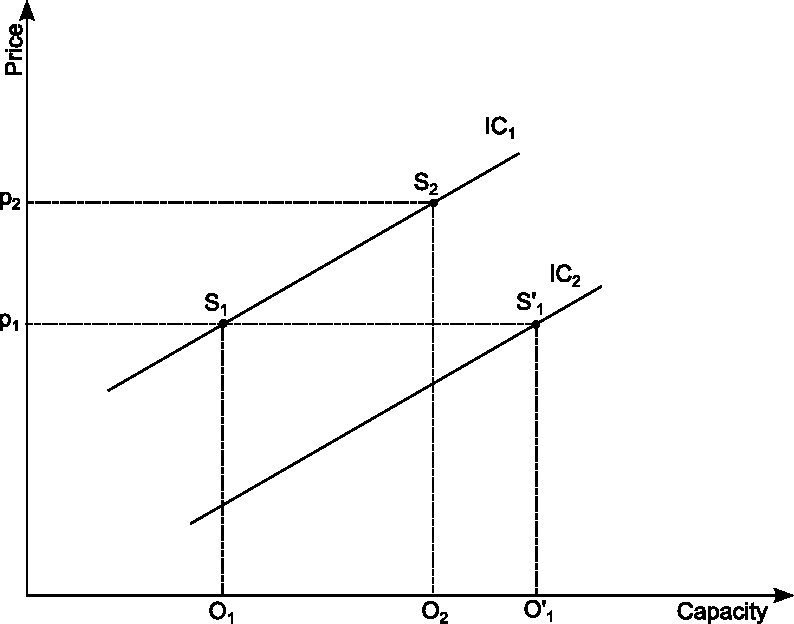
\includegraphics[scale=0.6]{pic/4.pdf} 
\caption{Indifference curves for equal satisfaction and utility}
\label{utility}
\end{figure}

\begin{equation}
U(p,O)=U_0-\gamma p+\delta O
\label{utilityfunc}
\end{equation}
 
where $p$, $O$, and $U_0$ are price, capacity and limiting value of satisfaction level respectively, and $\gamma$ and $\delta$ are coefficients. Following  equation~\ref{utilityfunc}, two indifference curves, $IC_{1}$ and $IC_{2}$ that represent equal satisfaction and utility are shown in Figure~\ref{utility}. To maintain same satisfaction level, if price $p$ is increased from $p_1$ to $p_{2}$ capacity must be increased from $O_1$ to $O_{2}$. Furthermore, the satisfaction of customers improves when they get more than what they paid for to the provider and thus, customer's satisfaction level changes from $S_1$ at $IC_{1}$ to $S_{1}^{'}$ at $IC_{2}$. 
%Customer's satisfaction level improves if customerjust need to pay price $p_i$ with a response time $t_{ai}$, point A is intersection point and satisfaction of customer i goes up because of IC1 alternating to ICm2.


%We assume one could provider can just control a type relationship of p and t, so from the graph, only one curve can reflect service quality of a could provider. Obviously, we can get a liner function to describe the relationship between price and response time without satisfaction U.

%
%\begin{equation}
%p=- t-\beta
%\end{equation}
%We call this function is contract function, because once cloud provider knew the service price p then can use it to determine response time t or vice versa. 

%For example,   modelled by following function:
%Figure \ref{figure4} shows the procedure of changing, 
%\begin{figure}[!t]
%\centering
%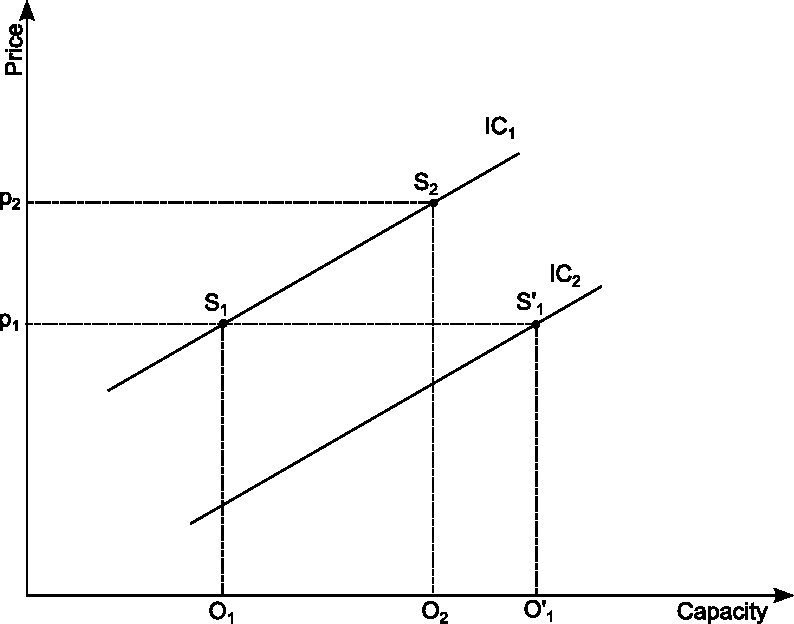
\includegraphics[width=2.5in]{pic/4.png}
%\caption{Basic Frame of the system}
%\label{figure4}
%\end{figure}


\subsubsection{Retention Action Policy}
%
%\begin{figure}[!t]
%\centering
%\includegraphics[width=2.5in]{pic/3.png}
%\caption{Basic Frame of the system}
%\label{figure3}
%\end{figure}



In our proposed retention action policy, RC is the amount of revenue that cloud service provider is willing to sacrifice. Since higher user churn rate demands for higher investment on user retention RC varies with churn rate $r$ according to following equation,

\begin{equation}
RC(r )= \varphi rp
\label{eq:retention}
\end{equation}

%\begin{equation}
%RC(r_c )= \begin{cases}\varphi r_c, & \mbox{if } 0 \leq rs_c \leq 0.1 \\{r_c}^{\log_{0.1}^⁡\varphi}, & \mbox{if } 0.1<r_c<1 \end{cases}
%\end{equation}

where $\varphi$ is a coefficient that establishes are linear relationship between churn rate and revenue. The amount of revenue to retain some customer $i$ is governed by its Retention Index (RI) which is given as
\begin{equation}
 RI_i=V_i *D_i 
\label{fixed}
\end{equation}

where $D_i$ and $V_i$ are degree of churn ($(0<D_i<1 )$) and value of customer $i$ respectively. Value of customer depends on summation of $P_u$, the revenue paid by customer at every time instant $u$ to cloud service provider. Therefore,  $V_i= \sum_{u=1}^U P_u$

Finally, retention cost $RC_{i}$ which is amount of revenue  a cloud service provider sacrifices on retaining a churner $i$ is decided according to following equation: 
\begin{equation}
RC_i=\dfrac{RC*RI_i}{\sum_{i=1}^n RI_i} 
\label{fixed}
\end{equation}

%The service provider agrees to give a fixed value on RA for all customers, but different people couldn't get a same value RA from this service provider, they need to distribute this RA based on the following strategy. For a particular customer, here we set up a . Index i indicates a particular customer i, and $V_i$ is her value, $D_i$ is her degree of churn $(0<D_i<1 )$. For the customer value V, we need to quantify it. If a particular customer is regular customer (not the first time to use the service of this provider), the value of this customer is $\sum_{u=1}^U P_u$ , u is history time she used this service and U is the total times she used, $P_u$ is how much money she paid for cloud provider at history time u, summarizing these payments that we can get this customer's value. However, except regular customers, a cloud provider can have some new customers, so we couldn't get their history records, that meaning $D_i$ of this customer is unknown. For dealing with this situation, we assume $D_i$ is equal to churner rate $r_c$ which cloud provider had known from statistics. 


%\subsubsection{Retention Action Policy, Ambulatory}

%In this case, the RA is a various values are given to every customer, so that service provider doesn't know how much they require on RA. But no matter how much they want to cost on RA, there is a unique principle which is the more important customers are the more RA those customers will get. 
%Ambulatory retention action policy does not put a cap on total revenue that cloud service providers sacrifice. Retention cost for different churners is computed individually. In our paper, ambulatory retention cost for a customer $i$ with retention index, $RI_i$ is given as below, 
%\begin{equation}
%RC_i=a*RI_i 
%\end{equation}
%where $a$ is a tunable parameter that can be set by cloud service provider.

%We have talked about Retention Action Index (RI) in the last section, so the RI can embody the degree of important for every customer, the customer has higher RI the more important for the cloud provider. Even though different companies or service providers could have different strategies on it, the mainstream idea should like this. In this case, each customer can get a RA which is 

\subsection{Virtual Machine Overhead}
%If we consider how the VMs place on PMs, there could have two models. The first one is using virtual CPUs in a single PM, so one physical CPU core can handle more than one VMs. However, this case is complex and may cause huge overhead, it includes both hyper-visor overhead and operation overhead. On the other way, one physical CPU core just handles one VM, so the number of running PMs could very high. Compare with this two strategies and our economic aim, the first placement method is much better than the second one. Figure X shows the basic structure.
In this work, two types of virtual machine overheads are considered, operation and interference.
\subsubsection{Operation Overhead}
Operation overhead is defined as VM hypervisor overhead caused by individual VMs. In this paper, Operation overhead of VM $i$ is modeled by a linear equation, $b*O_i$ where $O_i$ is capacity of VM $i$ and $b$ is constant for linear relation.
Therefore, total operation overhead $H_{j}^{o}$ on some PM $j$ is given as below,
\begin{equation}
H_{j}^{o}=\sum_{i=1}^n \theta_{ij} b O_i
\label{operationover}
\end{equation}
 where $n$ is the total numbers of VMs, $\theta_{ij}$ is 1 if  VM $i$ is located in PM $j$.

\subsubsection{Interference Overhead}
Since VMs placed on a PM share same memory and I/O resources each of them contribute to the degradation of overall utilization of the system~\cite{lin2012interference}. Clearly, such interference can cause thrashing and bring the PM utilization down at an exponential rate as more VMs are added. Therefore, interference overhead $H_{j}^{i}$ on PM $j$ is modelled as below:   
\begin{equation}
 H_{j}^{i}=c^{(\sum_{i=1}^n \theta_{ij} -1)}-1
\label{intereferenceover}
\end{equation}
where n is the total number of VMs , $\theta_{ij}$ is 1 if VM $i$ is placed on PM $j$. Note that a single VM does not cause interference overhead.

Combining equations~\ref{operationover} and~\ref{intereferenceover}, total VM overhead on some PM $j$  is given by $H_j$. 
\begin{equation}
H_j=\sum_{i=1}^m \theta_{ij} b O_i+(c^{(\sum_{i=1}^n \theta_{ij}-1)}-1), \ \ \sum_{i=1}^n \theta_{ij}-1 \geqslant 1
\label{totaloverhead}
\end{equation}
